\documentclass[11pt]{article}

\usepackage{amsmath,amssymb,mathtools}
\usepackage[margin=1in]{geometry}
\usepackage{enumitem}
\usepackage{xcolor}
\usepackage{microtype}
\usepackage{graphicx}
\usepackage{tikz,float}
\usepackage{subcaption}
\usepackage{amsthm}
\usepackage{hyperref}
\usepackage{array}
\usepackage{pgfplots}

\usetikzlibrary{shapes.geometric, arrows.meta, positioning, calc, decorations.markings}
\tikzset{
	block/.style={rectangle, draw, text width=6em, text centered, rounded corners, minimum height=10mm},
	sum/.style={circle, draw, node distance=1.5cm},
	line/.style={draw, -{Stealth[length=2.5mm, width=1.5mm]}}
}

\usepgfplotslibrary{groupplots}
\pgfplotsset{compat=1.18}

\pgfplotsset{
	myaxes/.style={
		axis lines=middle,
		axis line style={-latex},
		grid=major,
		grid style={gray!15},
		minor grid style={gray!35},
		xlabel style={at={(ticklabel* cs:1)}, anchor=north west},
		ylabel style={at={(ticklabel* cs:1)}, anchor=south east},
		every axis plot/.append style={thick}
	},
	myplotstyle/.style={
		width=14cm,
		height=7cm,
		axis lines=middle,
		axis line style={-Stealth},
		grid=both,
		minor tick num=1,
		major grid style={draw=gray!30},
		minor grid style={draw=gray!15},
		tick label style={font=\small, fill=white, inner sep=1.5pt},
		xlabel={$t$},
		ylabel={$x(t)$},
		xlabel style={anchor=north east, font=\small},
		ylabel style={anchor=south east, font=\small},
		samples=401,
	}
}

\newtheoremstyle{mynote}
{6pt}      % Space above
{6pt}      % Space below
{}          % Body font (normal, not italic)
{}          % Indent amount
{\bfseries} % Theorem head font
{.}         % Punctuation after theorem head
{.5em}      % Space after theorem head
{}          % Theorem head spec
\theoremstyle{mynote}
\newtheorem{definition}{Definition}
\newtheorem{proposition}{Proposition}
\newtheorem{example}{Example}
\newtheorem{remark}{Remark}
\newtheorem{theorem}{Theorem}
\newtheorem{corollary}{Corollary}

\newcommand{\T}{\mathcal{T}}
\newcommand{\R}{\mathbb{R}}
\newcommand{\Z}{\mathbb{Z}}
\newcommand{\C}{\mathbb{C}}
\newcommand{\conv}{\ast}
\newcommand{\dt}{\,\dd t}
\newcommand{\dd}{\mathrm{d}}
\newcommand{\imp}{\delta}
\newcommand{\sinc}[1]{\frac{\sin(\pi #1)}{\pi #1}}


\DeclareMathOperator{\rect}{rect}
\DeclareMathOperator{\Ev}{Ev}
\DeclareMathOperator{\Od}{Od}
\DeclareMathOperator{\sgn}{sgn}
\DeclareMathOperator{\step}{u}
\DeclareMathOperator{\tri}{tri}


\begin{document}
	% Reset figure counter for this lecture
	\renewcommand{\thefigure}{1.\arabic{figure}}
	
	% --- TITLE BLOCK ---
	\thispagestyle{empty}
	\noindent
	\begin{tabular*}{\textwidth}{l @{\extracolsep{\fill}} r}
		\textbf{Signals and Systems} & \textbf{Lecture 1} \\
		\textit{Dr. Ghandi Manasra and Ahmed Rabei} & \textit{Fall 2025} \\
	\end{tabular*}
	\hrule
	\vspace{0.4cm}
	\begin{center}
		\Large\textbf{Lecture 1: Introduction to Signals}
	\end{center}
	\vspace{0.4cm}
	
\section*{Reference}
	Oppenheim \& Willsky, \textit{Signals and Systems}, Chapter 1, Sections 1.0--1.2.1

	\section*{Review of Prerequisites}
	\begin{itemize}[noitemsep]
		\item Basic calculus and functions
		\item \textbf{Understanding of} complex numbers
		\item \textbf{Familiarity with} mathematical notation
		\item Engineering problem-solving approach
	\end{itemize}

	\section*{1.0 Welcome \& Introduction}
	
	\section*{1.1 What is a Signal?}
	\begin{definition}
		A \textbf{signal} is information that changes over time (or space). Mathematically, it is a function of one or more independent variables.
	\end{definition}
	
	\begin{itemize}[noitemsep]
		\item \textbf{Continuous-Time (CT):} \(x(t)\), \(t \in \R\).
		\item \textbf{Discrete-Time (DT):} \(x[n]\), \(n \in \Z\).
		\item Convention: use parentheses for CT, brackets for DT.
	\end{itemize}
	
	\section*{1.2 What is a System?}
	\begin{definition}
		A \textbf{system} is any process or operation that acts on a signal to produce another signal. It takes a signal, performs some operation, and outputs a new signal.
	\end{definition}
	
	\begin{itemize}[noitemsep]
		\item Systems can be physical (amplifier, filter) or abstract (algorithms in DSP).
		\item Systems can be modeled by an operator \(\T\{\cdot\}\):
		\[
		\text{Continuous-Time (CT):} \quad y(t) = \T\{x(t)\}, \qquad \text{Discrete-Time (DT):} \quad y[n] = \T\{x[n]\}.
		\]
	\end{itemize}
	\newpage
	\section*{1.3 Two Basic Types of Signals and Systems}
	
	\subsection*{1.3.1 Continuous-Time (CT) Signals and Systems}
	\begin{itemize}[noitemsep]
		\item \(x(t)\), \(t \in \R\).
		\item Defined for every instant of continuous time.
		\item Examples: analog audio, temperature variation, vibrations.
		\item Systems act on CT signals: \( y(t) = \T\{x(t)\} \).
		\[
		x(t) \longrightarrow \boxed{\quad CTS \quad} \longrightarrow y(t)
		\]
	\end{itemize}
	\begin{example}
		Consider a Gaussian pulse as a CT signal:
		\begin{figure}[H]
			\centering
			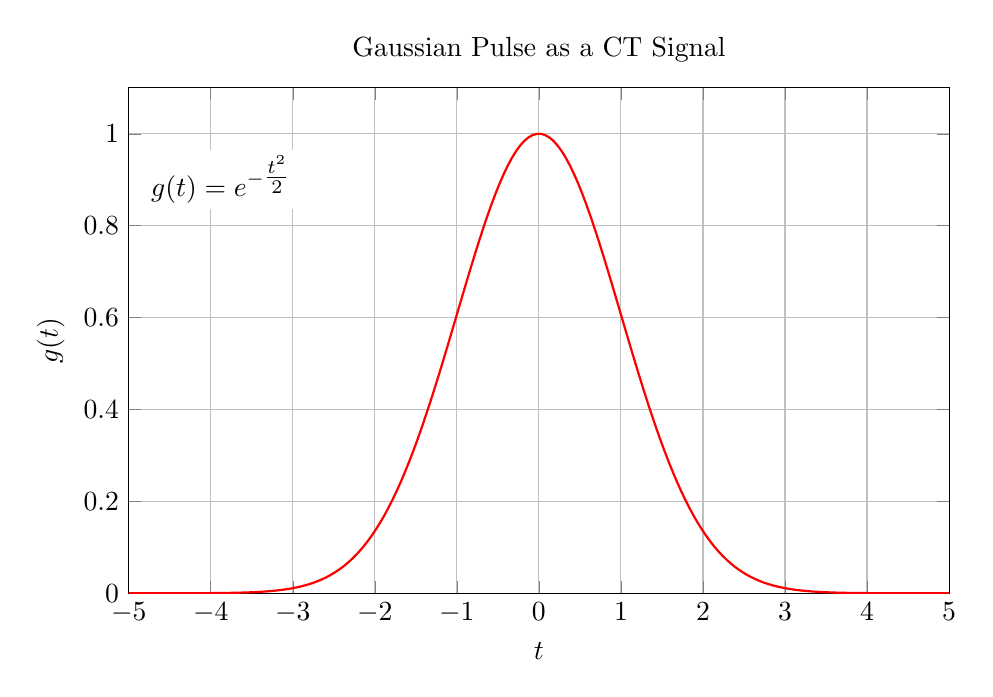
\begin{tikzpicture}
	\begin{axis}[
		title={Gaussian Pulse as a CT Signal},
		xlabel={$t$},
		ylabel={$g(t)$},
		xmin=-5, xmax=5,
		ymin=0, ymax=1.1,
		grid=major,
		width=12cm,
		height=8cm,
		]
		\addplot[
		color=red,
		thick,
		domain=-5:5,
		samples=200,
		]
		{exp(-x^2 / 2)};
		\node[anchor=west, fill=white, inner sep=2pt] at (axis cs:-4.8,0.9) 
		{$g(t) = e^{-\tfrac{t^2}{2}}$};
	\end{axis}
\end{tikzpicture}

			\caption{Gaussian pulse as continuous-time signal example.}
			\label{fig:gaussian_pulse}
		\end{figure}
	\end{example}
	
	\subsection*{1.3.2 Discrete-Time (DT) Signals and Systems}
	\begin{itemize}[noitemsep]
		\item \(x[n]\), \(n \in \Z\).
		\item Defined only at specific, discrete points.
		\item Systems: \( y[n] = \T\{x[n]\} \).
		\[
		x[n] \longrightarrow \boxed{\quad DTS \quad} \longrightarrow y[n]
		\]
		\item Examples: sampled audio, stock prices, digital images.
		\item Often arise from sampling CT signals.
	\end{itemize}
	\newpage
	\begin{example}
		Consider a sampled Gaussian pulse as a DT signal:
		\begin{figure}[H]
			\centering
			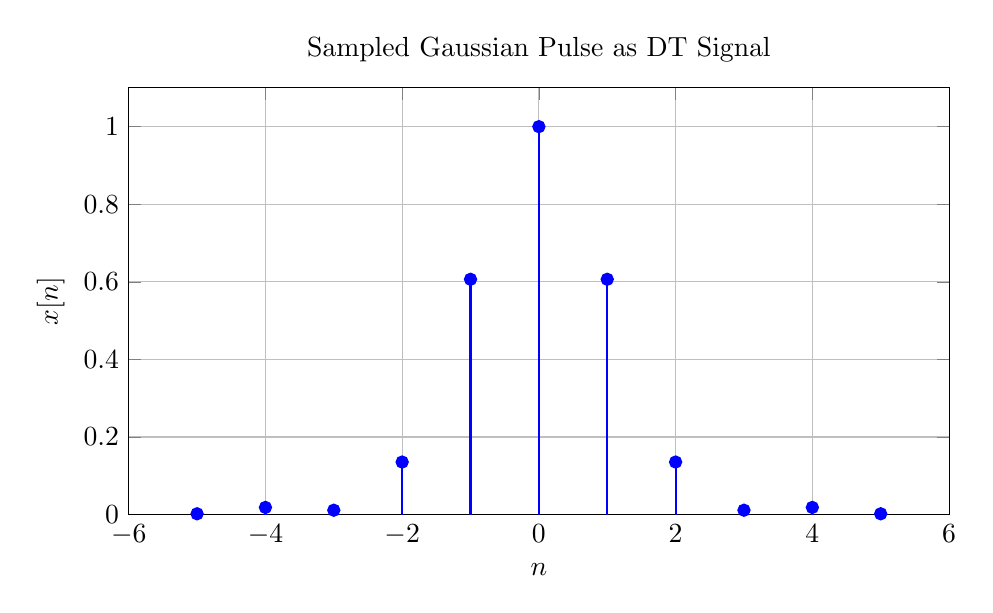
\begin{tikzpicture}
	\begin{axis}[
		title={Sampled Gaussian Pulse as DT Signal},
		xlabel={$n$},
		ylabel={$x[n]$},
		xmin=-6, xmax=6,
		ymin=0, ymax=1.1,
		grid=major,
		width=12cm,
		height=7cm,
		]
		\addplot[
		ycomb,
		blue,
		thick,
		mark=*,
		mark options={fill=blue},
		]
		coordinates {
			(-5,0.0019) (-4,0.0183) (-3,0.0111) (-2,0.1353)
			(-1,0.6065) (0,1) (1,0.6065) (2,0.1353)
			(3,0.0111) (4,0.0183) (5,0.0019)
		};
	\end{axis}
\end{tikzpicture}

			\caption{Sampled Gaussian pulse as discrete-time signal.}
			\label{fig:sampled_gaussian}
		\end{figure}
	\end{example}
	
	\section*{1.4 Deterministic vs Random Signals}
	\begin{itemize}[noitemsep]
		\item \textbf{Deterministic:} Completely predictable, e.g. \(x(t) = \cos(2\pi t)\).
		\item \textbf{Random:} Unpredictable, described by statistics (mean, variance, spectrum). Example: thermal noise.
		\item Course focus: deterministic signals, but real-world signals often contain randomness.
	\end{itemize}
	
	\section*{1.5 Energy and Power of Signals}
	
	The energy and power of a signal provide fundamental measures of its "strength" or "intensity." These definitions have deep physical significance: for a voltage signal \(x(t)\) across a 1-ohm resistor, the energy represents the total energy dissipated, and the power represents the average rate of energy dissipation.
	
	\subsection*{Formal Definitions (CT case)}
	\[
	E_\infty = \int_{-\infty}^\infty |x(t)|^2 \dt, 
	\quad 
	P_\infty = \lim_{T \to \infty} \frac{1}{2T} \int_{-T}^T |x(t)|^2 \dt
	\]
	
	\subsection*{Discrete-Time Analogs}
	\[
	E_\infty = \sum_{n=-\infty}^\infty |x[n]|^2,
	\quad
	P_\infty = \lim_{N \to \infty} \frac{1}{2N+1}\sum_{n=-N}^N |x[n]|^2
	\]
	
	\subsection*{Key Categories}
	\begin{itemize}[noitemsep]
		\item Energy Signal: \(0 < E_\infty < \infty, \; P_\infty = 0\).
		\item Power Signal: \(E_\infty = \infty, \; 0 < P_\infty < \infty\).
	\end{itemize}
	
	\subsection*{Example 1: Rectangular Pulse (Energy)}
	\[
	x(t) = \begin{cases}
		1 & -1 \leq t \leq 1 \\
		0 & \text{otherwise}
	\end{cases}
	\quad\Rightarrow\quad
	E_\infty = \int_{-1}^1 1\,\dt = 2
	\]
	
	\subsection*{Example 2: Cosine Wave (Power)}
	\[
	x(t) = A \cos(\omega_0 t)
	\]
	\[
	E_\infty \to \infty, \qquad P_\infty = \tfrac{A^2}{2}
	\]
	
	\subsection*{Signals That Are Neither}
	\begin{itemize}[noitemsep]
		\item Condition: \(E_\infty = \infty,\; P_\infty = \infty\).
		\item Example: Ramp signal 
		\[
		x(t) = t u(t) =
		\begin{cases}
			t, & t \geq 0 \\
			0, & t < 0
		\end{cases}
		\]
	\end{itemize}
	
	\section*{1.6 Transformations of Signals}
	\begin{itemize}[noitemsep]
		\item \textbf{Time Shift:} \(x(t-t_0)\) or \(x[n-n_0]\). Delay if \(t_0 > 0\), advance if \(t_0 < 0\).  
		\item \textbf{Time Reversal:} \(x(-t)\), \(x[-n]\). Reflection about zero.  
		\item \textbf{Time Scaling:} \(x(at)\). If \(|a| > 1\), compression; if \(0 < |a| < 1\), expansion.  
		\item \textbf{Combined:} \(x(\alpha t+\beta)\). To avoid ambiguity, always factor as \(x(\alpha(t + \beta/\alpha))\).
		\begin{itemize}
			\item \textbf{Clear method:} Factor to get \(x(\alpha(t + \beta/\alpha))\), then apply transformations in order: first shift by \(-\beta/\alpha\), then scale by \(\alpha\).
		\end{itemize}
	\end{itemize}
	
	\section*{Summary and Next Lecture}
	\begin{itemize}[noitemsep]
		\item Defined signals, systems, CT vs DT signals.
		\item Deterministic vs random signals.
		\item Energy and power classification.
		\item Time-domain transformations.
		\item \textbf{Next time:} Elementary signals, periodicity, and symmetry.
	\end{itemize}
	
\end{document}